\section{Final Notes}
\textbf{1.} It was required to reflect the status of the robot in the feedback. In our program, the server sends feedback only when the robot is moving and detecting, so there is only one type of status and one type of feedback message. The feedback content still reflects the status of the robot since it contains the current position of the robot (indicating movement and position updates) and the lists of cylinders (indicating detection).\\\\

\textbf{2.} In the video, we can observe occasional false positives in the feedback of the first goal sent, but memorizing the largest group of cylinders helps the server to rectify these errors. It would be highly improbable for the algorithm to produce multiple errors simultaneously. Additionally, different values for the position, orientation, and feedback flag yield various outputs, demonstrating the robot's correct behavior in response to these parameters.\\\\

\textbf{3.} In the folder \texttt{./Other documentations/assignment\_1}, you will find the file \texttt{refman.pdf}, which provides further explanation of the steps to execute in order to start the program and a more comprehensive documentation of the code.\\ 
Additionally, in the folder \texttt{./Other documentations/assignment\_1/html}, you will find the file \texttt{index.html}, which contains an interactive representation of the documentation. It is recommended to review both sources for a complete understanding of the work done.\\\\

\textbf{4.} As highlighted in the image (see Figure \ref{fig:example}), we are aware that our method, although functional, might have limitations if the robot approaches objects too closely. Currently, the navigation system prevents the robot from getting too close to objects. However, if it were to get too close, the identified centers of the objects could be misaligned or even, in extreme cases, not be correctly identified if below a certain threshold.

\begin{figure}[h]
    \centering
    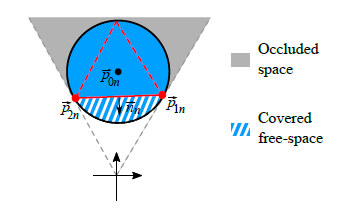
\includegraphics[width=0.5\textwidth]{./images/detection/circle-extraction.PNG} % Replace example-image with your image file
    \caption{Example Image of the space around the objects.}
    \label{fig:example}
\end{figure}

%\bibliographystyle{plain} % We choose the "plain" reference style
%\bibliography{bibliography}